\documentclass[aspectratio=169,11pt]{beamer}

\usepackage{graphicx}
\usepackage{tikz}
\usetikzlibrary{positioning,arrows.meta}
\usepackage{xcolor}
\usepackage{booktabs}
\usepackage{tabularx}
\usepackage{array}
\usepackage{ragged2e}

\definecolor{GEUBlue}{RGB}{20,55,105}
\definecolor{GEULightBlue}{RGB}{238,244,251}
\definecolor{GEUGrey}{RGB}{90,90,90}
\definecolor{GEULightGrey}{RGB}{245,246,248}

\usetheme{default}
\setbeamertemplate{navigation symbols}{}
\setbeamertemplate{blocks}[rounded][shadow=false]
\setbeamercolor{normal text}{fg=black,bg=white}
\setbeamercolor{frametitle}{fg=GEUBlue}
\setbeamercolor{structure}{fg=GEUBlue}
\setbeamercolor{block title}{fg=GEUBlue,bg=GEULightBlue}
\setbeamercolor{block body}{fg=black,bg=GEULightBlue}
\setbeamerfont{frametitle}{size=\Large,series=\bfseries}

% Replace with the actual logo filename (place graphicera_logo.png next to this .tex file)
\newcommand{\GEULogo}{graphicera_logo.png}

% Header and footer
\setbeamertemplate{headline}{%
  \begin{tikzpicture}[remember picture,overlay]
    \node[anchor=north east,xshift=-0.30cm,yshift=-0.12cm]
      at (current page.north east)
      {\includegraphics[height=0.62cm]{\GEULogo}};
  \end{tikzpicture}
  \vspace{0.72cm}
}
\setbeamertemplate{frametitle}{%
  \vspace{0.03cm}
  \insertframetitle\par
  \vspace{0.04cm}
  \textcolor{GEUBlue}{\rule{\textwidth}{0.9pt}}
  \vspace{0.03cm}
}
\setbeamertemplate{footline}{%
  \leavevmode
  \hbox{%
  \begin{beamercolorbox}[wd=.82\paperwidth,ht=0.32cm,dp=0.10cm,leftskip=.3cm]{author in head/foot}
    \tiny Department of Computer Science \& Engineering | Graphic Era (Deemed to be University)
  \end{beamercolorbox}%
  \begin{beamercolorbox}[wd=.18\paperwidth,ht=0.32cm,dp=0.10cm,rightskip=.3cm]{date in head/foot}
    \hfill\tiny\insertframenumber/\inserttotalframenumber
  \end{beamercolorbox}}
}

\newcommand{\smallnote}[1]{\vspace{0.08cm}{\scriptsize\color{GEUGrey}#1}}

\title{\textbf{Project-Based Learning}\\[2mm]\large Phase-I Evaluation}
\author{\textbf{ML-Core: A C++ Implementation of Fundamental Machine Learning Algorithms}\texorpdfstring{\\}{, }Team ID: T170}
\institute{Department of Computer Science \& Engineering\\Graphic Era (Deemed to be University), Dehradun}
\date{Academic Session 2026--27}

\begin{document}

% 1
\begin{frame}[plain]
\begin{tikzpicture}[remember picture,overlay]
\draw[GEUBlue,line width=3pt] (current page.north west) -- (current page.north east);
\node[anchor=north east,xshift=-0.45cm,yshift=-0.35cm] at (current page.north east)
{\includegraphics[height=1.0cm]{\GEULogo}};
\node[align=center,text width=.84\paperwidth] at ([yshift=.25cm]current page.center)
{{\color{GEUBlue}\fontsize{26}{30}\selectfont\bfseries PROJECT-BASED LEARNING}\\[3mm]
 {\fontsize{18}{22}\selectfont PHASE-I EVALUATION}\\[7mm]
 {\color{GEUGrey}\Large\bfseries ML-Core: A C++ Implementation of\\Fundamental Machine Learning Algorithms}\\[3mm]
 {\color{GEUBlue}\normalsize Team ID: T170}};
\node[align=center,anchor=south,yshift=.42cm] at (current page.south)
{\bfseries Department of Computer Science \& Engineering\\
Graphic Era (Deemed to be University), Dehradun\\[-1mm]
\scriptsize Academic Session 2026--27};
\end{tikzpicture}
\end{frame}

% 2
\begin{frame}{Team \& Mentor Details}
\begin{columns}[T,totalwidth=\textwidth]
\column{.48\textwidth}
\begin{block}{Team Information}
\begin{tabular}{@{}ll@{}}
\textbf{Team ID:} & DSCPP-III-2026-T170\\
\textbf{Team Name:} & ML Core\\
\textbf{Semester:} & 3rd\\
\textbf{Section:} & ML2,DS1,DS2\\
\textbf{Domain:} & Machine Learning 
\end{tabular}
\end{block}
\column{.48\textwidth}
\begin{block}{Team Members}
1.\quad Shubhangani Kotiyal -- 2510370294\\ \scriptsize(Team Lead)\\[1mm]
\normalsize 2.\quad Ishanaya Agarwal -- 2510380249\\
3.\quad Harshita Joshi -- 2510380118
\end{block}
\end{columns}
\vspace{2mm}
\begin{block}{Mentor}
Dr. Hriday Kumar Gupta
\hfill
\textbf{Interactions completed:} 2
\end{block}
\end{frame}

% 3
\begin{frame}{Problem Statement \& Motivation}
\begin{block}{Problem Statement}
High-level machine learning libraries such as Scikit-learn and TensorFlow let users train models like K-Means or SVM through a single function call, hiding the underlying mathematics -- centroid updates, hyperplane computation, gradient descent -- behind a black box. This project builds six classical ML algorithms from scratch in C++ to make that mathematics fully transparent.
\end{block}
\vspace{2mm}
\begin{columns}[T,totalwidth=\textwidth]
\column{.48\textwidth}
\textbf{\color{GEUBlue}Motivation}
\begin{itemize}\itemsep2pt
\item High-level libraries abstract away core computations (matrix ops, gradients, distance metrics)
\item Limits understanding of memory management \& computational efficiency needed for resource-constrained systems
\item Existing C/C++ ML libraries (mlpack, dlib, Shark) target performance, not learning
\end{itemize}
\column{.48\textwidth}
\textbf{\color{GEUBlue}Target Users / Stakeholders}
\begin{itemize}\itemsep2pt
\item CS / ML students learning algorithm internals
\item Self-learners without access to production tooling
\item Embedded / resource-constrained systems developers
\end{itemize}
\end{columns}
\end{frame}

% 4
\begin{frame}{Objectives}
\textbf{\color{GEUBlue}Project Objectives}
\vspace{2mm}
\begin{enumerate}\itemsep5pt
\item Implement six classical ML algorithms -- Linear Regression, SVM, KNN, K-Means, Hierarchical Clustering, and PCA -- from scratch in C++.
\item Build a shared utility library for matrix operations, distance metrics, and CSV parsing.
\item Design each algorithm as an independent C++ module, with a separate source file for each algorithm.
\item Validate correctness of each implementation against Python's Scikit-learn.
\item Produce visual output (trend lines, decision boundaries, clusters, dendrograms) for each algorithm.
\end{enumerate}
\vfill
\begin{center}
\colorbox{GEULightBlue}{\parbox{.85\textwidth}{\centering
\textbf{Key Objective:} Deliver six working, from-scratch ML implementations in C++, each verified for correctness against Scikit-learn.}}
\end{center}
\end{frame}

% 5
\begin{frame}{Proposed Solution}
\begin{columns}[T,totalwidth=\textwidth]
\column{.48\textwidth}
\textbf{\color{GEUBlue}Proposed Approach}
\begin{enumerate}\itemsep3pt
\item Data Layer -- CSV parsing \& cleaning into numeric arrays
\item Core Utility Layer -- matrix operations, distance/gradient/eigen functions
\item Algorithm Module Layer -- six independent algorithm implementations
\item Testing -- hand-calculated small datasets, then comparison vs.\ Scikit-learn
\item Output Layer -- validation, comparison \& visualization
\end{enumerate}
\column{.48\textwidth}
\textbf{\color{GEUBlue}Key Features}
\begin{itemize}\itemsep3pt
\item Six ML algorithms built from scratch in C++
\item Shared, reusable core utility library
\item Modular architecture -- each algorithm independent \& testable
\item Correctness verified against Scikit-learn
\item Visual output: trend lines, cluster maps, dendrograms
\end{itemize}
\end{columns}
\vfill
\smallnote{No external ML libraries are used; algorithms are implemented in C++ with the standard library.}
\end{frame}

% 6
\begin{frame}{Integration of PBL Course Concepts}
\scriptsize
\begin{center}
\renewcommand{\arraystretch}{1.25}
\begin{tabularx}{.96\textwidth}{@{}>{\bfseries}p{3.0cm}X p{3.3cm}@{}}
\toprule
Course & Concepts Applied & Project Module\\
\midrule
Data Structures & Vectors and matrices for dataset representation; records for data; searching \& sorting for nearest-neighbour selection (KNN); distance-based computations for clustering; tree-like dendrogram construction (Hierarchical Clustering) & Core Utility Layer \& Algorithm Modules\\
\midrule
OOPs with C++ & C++ classes and encapsulation for algorithm state; modular design with one source file per algorithm; reusable functions for shared operations & Algorithm Module Layer design\\
\bottomrule
\end{tabularx}
\end{center}
\vfill
\begin{center}
\colorbox{GEULightBlue}{\parbox{.86\textwidth}{\centering
\textbf{Requirement:} Demonstrate meaningful integration of both subjects in \textbf{one} project.}}
\end{center}
\end{frame}

% 7
\begin{frame}{System Architecture / Workflow}
\begin{center}
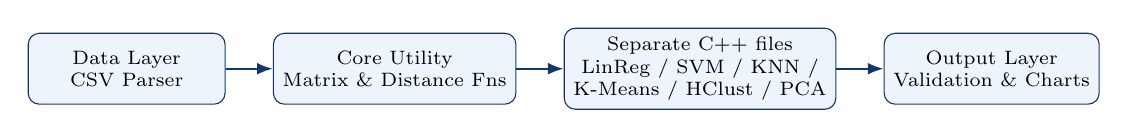
\begin{tikzpicture}[
node distance=6mm,
box/.style={rectangle,rounded corners,draw=GEUBlue,fill=GEULightBlue,
minimum width=2.5cm,minimum height=9mm,align=center,font=\scriptsize},
arrow/.style={-{Latex[length=2mm]},thick,draw=GEUBlue}
]
\node[box] (a) {Data Layer\\CSV Parser};
\node[box,right=of a] (b) {Core Utility\\Matrix \& Distance Fns};
\node[box,right=of b] (c) {Separate C++ files\\LinReg / SVM / KNN /\\K-Means / HClust / PCA};
\node[box,right=of c] (d) {Output Layer\\Validation \& Charts};
\draw[arrow] (a)--(b); \draw[arrow] (b)--(c); \draw[arrow] (c)--(d);
\end{tikzpicture}
\end{center}
\vspace{5mm}
\begin{columns}[T,totalwidth=\textwidth]
\column{.48\textwidth}
\textbf{\color{GEUBlue}Major Components}
\begin{itemize}\itemsep2pt
\item CSV Parser \& Data Layer
\item Core Utility Library (matrix ops, distance/math functions)
\item Six Algorithm Modules (Linear Regression, SVM, KNN, K-Means, Hierarchical Clustering, PCA)
\end{itemize}
\column{.48\textwidth}
\textbf{\color{GEUBlue}Data / Control Flow}
\begin{itemize}\itemsep2pt
\item Raw CSV is parsed \& cleaned into numeric data
\item Data is passed to the selected algorithm module via shared utilities
\item Output layer validates results against Scikit-learn and generates charts
\end{itemize}
\end{columns}
\end{frame}

% 8
\begin{frame}{Technology Stack \& Methodology}
\begin{columns}[T,totalwidth=\textwidth]
\column{.48\textwidth}
\begin{block}{Technology Stack}
\begin{itemize}\itemsep2pt
\item Programming: C++ (standard library)
\item Database: None -- flat CSV files
\item Tools: Python + Scikit-learn (verification only)
\item IDE: VS Code
\item Version Control: Git / GitHub
\end{itemize}
\end{block}
\column{.48\textwidth}
\begin{block}{Development Methodology}
\begin{enumerate}\itemsep2pt
\item Preparation (theory \& math study)
\item Core Utility Development
\item Algorithm Implementation
\item Testing \& Validation vs.\ Scikit-learn
\item Finalization \& Documentation
\end{enumerate}
\end{block}
\end{columns}
\vfill
\begin{center}
\smallnote{No external ML libraries are used; correctness is checked by cross-verifying against Scikit-learn.}
\end{center}
\end{frame}

% 9
\begin{frame}{Initial Progress \& Team Contribution}
\begin{columns}[T,totalwidth=\textwidth]
\column{.44\textwidth}
\textbf{\color{GEUBlue}Progress Achieved}
\begin{itemize}\itemsep3pt
\item Literature \& background study of all six algorithms completed
\item Requirements finalized
\item Four-layer modular architecture designed
\item Core utilities \& algorithm coding not yet started (planning/design stage)
\end{itemize}
\column{.52\textwidth}
\textbf{\color{GEUBlue}Individual Contribution}
\vspace{2mm}
\scriptsize
\begin{tabularx}{\textwidth}{@{}p{2.3cm}p{1.6cm}X@{}}
\toprule
Member & Role & Contribution\\
\midrule
Shubhangani Kotiyal & Team Lead & Coordination; Linear Regression \& SVM modules\\
Ishanaya Agarwal & Developer & KNN \& K-Means modules\\
Harshita Joshi & Developer & Hierarchical Clustering \& PCA modules\\
\bottomrule
\end{tabularx}
\end{columns}
\end{frame}

% 10
\begin{frame}{Roadmap, Expected Outcomes \& References}
\begin{columns}[T,totalwidth=\textwidth]
\column{.48\textwidth}
\textbf{\color{GEUBlue}Roadmap}
\begin{enumerate}\itemsep3pt
\item Phase-I: Proposal \& Design
\item Phase-II: Core Utilities \& Algorithm Development
\item Phase-III: Testing, Validation \& Final Demo
\end{enumerate}
\vspace{2mm}
\textbf{\color{GEUBlue}Expected Outcomes}
\begin{itemize}\itemsep2pt
\item Six working, from-scratch ML algorithms in C++
\item Correctness verified against Scikit-learn
\item Visual results: trend lines, clusters, dendrograms
\item Complete documentation of math \& implementation
\end{itemize}
\column{.48\textwidth}
{\scriptsize\setlength{\leftmargini}{10pt}
\textbf{\color{GEUBlue}References}
\begin{enumerate}\itemsep1pt
\item Bishop, \emph{Pattern Recognition \& ML} (2006)
\item Hastie et al., \emph{Elements of Stat.\ Learning} (2009)
\item Cortes \& Vapnik, \emph{Support-Vector Networks} (1995)
\item MacQueen, \emph{Classification \& Analysis} (1967)
\item Stroustrup, \emph{The C++ Prog.\ Language}, 4th ed. (2013)
\item Pedregosa et al., \emph{Scikit-learn} (JMLR, 2011)
\end{enumerate}}
\vspace{2mm}
\begin{center}
\colorbox{GEUBlue}{\parbox{.9\linewidth}{\centering\color{white}\textbf{Thank You}\\Questions \& Suggestions}}
\end{center}
\end{columns}
\end{frame}

\end{document}
